\chapter{\library{Lantern}: Data-driven Acoustic Echo Retrieval}\label{ch:lantern}

\marginpar{%
    \footnotesize
    \textbf{Keywords:} Acoustic Echo Retrieval, TDOA Estimation, Supervised Learning, Deep Learning, Robust Regression.
    \\\textbf{Resources:}
    \begin{itemize}
        \item \href{https://ieeexplore.ieee.org/document/8683534}{ICASSP2018 Paper}
        \item \href{https://github.com/Chutlhu/MIRAGE}{Code}
        \item \href{https://sigport.org/documents/mirage-2d-sound-source-localization-using-microphone-pair-augmentation-echoes}{ICASSP2018 Poster}
    \end{itemize}
}
\newthought{Synopsis} \synopsisChLantern

\mynewline
Deep learning notions are personal digestion of materials available in standard machine learning textbooks, such as~\citeonly{bishop2006pattern,goodfellow2016deep}, and the recent comprehensive work of~\citeonly{purwins2019deep} oriented to audio signal processing.
Instead, in the remaining sections, we will present part of the previously published work~\cite{di2019mirage} and a technical report~\cite{di2019honda} and on going research.

\mynewline
It is essential to say that the approaches presented here are part of a first investigation in echo-aware \ac{SSL}.
Therefore they are profoundly interconnected with~\cref{ch:mirage}, which can be considered a following up of the earlier work~\citeonly{gaultier2017vast} authored by colleagues.
With that being said, we will mainly focus on a simple yet common scenario where we estimate only the first and strongest echo.
The generalization to multiple echoes will only be discussed as future work.

\section{Introduction}\label{sec:lantern:intro}
Recently \acfp{DNN} has captured the attention of many research fields due to recent advances that allow for faster implementation and training, as well as for achieving considerable performance improvement.
Therefore, \acp{DNN}s have been widely used in many domains.
They belong to the class of \textit{supervised} learning or \textit{data-driven} models, where the training step is performed on labeled data, namely input-output pairs.
The inclusion of these models in audio signal processing tasks has meant a considerable improvement in the performance, mainly audio and music source separation, speech enhancement, and source localization (see related sections in~\cref{ch:application}).
\\Moreover, with respect to traditional machine learning methods, the use of deep learning models presents other advantages.
They are flexible and adaptable across tasks; for instance, \acf{CNN}-based models from Computer Vision can be adapted for audio source separation (\eg/,~\citeonly{xiao2016deep, sainath2017multichannel, perotin2018crnn}), and for source localization(\eg/, ~\citeonly{chakrabarty2017broadband,vesperini2018localizing,nguyen2018autonomous,salvati2018exploiting}).
Furthermore, \acp{DNN}s reduce --- even remove --- the step of designing hand-crafted features, by including the feature learning as part of the learning process.
\\Other
\marginpar{
    \itshape\footnotesize
    At first, the \acf{GLLiM} framework was considered to address the \ac{AER} problem. Then, we oriented our attention towards \ac{DNN} models, which gave already satisfactory results.
    It seemed that the local-linearity assumption of \ac{GLLiM} was in contrast with the highly non-linear nature of the mapping between echoes and observation.
    Nevertheless, we recognize other benefits in using the \ac{GLLiM} framework, which cannot be found in the \ac{DNN}-based approach, such as, the ability to generalize to missing data at the input or including prior statistical knowledge in the model.
} supervised learning methods have been proposed in audio processing literature, such as \ac{GMM}-based frameworks~\citeonly{laufer2013relative,deleforge2015acoustic,gaultier2017vast}.
This framework allows to build power models based on probabilistic prior knowledge and are competing with \ac{DNN} models in case of a small training dataset.
However, they ofter require a strong assumption of the nature of the mapping between input-output pairs, such as (local-)linearity or independence between the variables.

\mynewline
The use of supervised learning models (not only the \ac{DNN}), presents some disadvantages.
One of the most relevant ones is their dependence on annotated data. It results in a significant bottleneck in audio signal processing tasks because collecting and annotating comprehensive real-world acoustic data is not trivial, since it requires proper tools, expertise, and time.
To overcome this issue, a standard approach nowadays is to used training data generated by simulators.
We will refer to this approach as \textit{virtually supervised learning} and it provides great versatility, for instance:
\begin{itemize}
    \item many different acoustic condition can be include in the training data,\\\eg/, different \acf{RT$_{60}$} and \acf{SNR} levels;
    \item a precise (up to computer precision) annotation of the data come directly,\\\eg/ spatial, temporal information of the audio scene events;
    \item and finally, the data can be potentially re-used for different application,\\\eg/, localization, separation, diarization, \etc/;
\end{itemize}
Besides, the solutions obtained in a data-driven fashion suffer from bias depending on the dataset used and may not generalize to real-world scenarios.
Interestingly, the work in~\citeonly{nguyen2018autonomous} discusses an automatic approach for collecting, annotating data automatically as a pre-calibration step.
However, this approach is possible only with specific technologies and applications (the authors programmed a humanoid robot equipped with a binaural hearing system that automatically builds a training set).
The following section will gives a quick overview of relevant models used in our work.

\section{Deep Learning Model}\label{sec:lantern:dnn}

\subsection{Multi-layer perceptions}\label{subsec:lantern:mlp}
\acf{MLP} are simple and basic modules of \ac{DNN} and are also known as \textit{fully-connected} or \textit{dense layers}.
They consist of a sequence of layer, each of which defined by an affine transformation followed by a non-linearity function:
\begin{equation*}
    \bfy = f(\bfW \bfx + \bfb)
    ,
\end{equation*}
where
\newcommand{\Din}{\ensuremath{D_{\text{in}}}}
\newcommand{\Dout}{\ensuremath{D_{\text{out}}}}
\begin{itemize}
    \item $\bfx\in\bbR^{\Din}$ is the input,
    \item $\bfy\in\bbR^{\Dout}$ is the output,
    \item and $\bfb\in\bbR^{\Dout}$ and $\bfW\in\bbR^{\Dout \times \Din}$ are the \textit{bias vector} and the \textit{weight matrix}, respectively.
\end{itemize}
The function $f(\cdot)$ is a non-linear \textit{activation} function, which allows the model to learn non-linear structures.
Models built with these layers are typically used to map the input to a representation space where problems (\eg/, classification, and regression) can be addressed more easily.
The main drawback of these simple models is that they are not invariant to scaled or shifted input.
Since in audio data, gain, temporal, and frequency variations are common, they not suitable.
Nevertheless, \acp{MLP} are used in combination with other type of layers, such as \acfp{CNN}, \acfp{RNN}.

\newthought{Non-linear activation functions} are one of the key feature of \acp{DNN}.
Thanks to these, the model can achieve more \textit{expressive power} with respect to linear models~\citeonly{goodfellow2016deep}.
Without these functions, it can be shown that the composition of affine transformations is equivalent to a single affine transformation.
Therefore, the activation functions make the model capable of account for more complex relationships between the input and the output than an affine transformation.
Typical examples of these functions are, for instance, hyperbolic tangent, the Sigmoid function, and \acf{ReLU}.

\subsection{Convolutional neural networks}\label{subsec:lantern:cnn}
The \ac{CNN} consists of convolutional layers that have been introduced to overcome some limitations of the simple linear ones.
In a nutshell, they consist of learnable kernel functions that are convolved with their input.
Therefore, they are characterized by
\begin{itemize}
    \item shift-invariance property, and can be used to reduce the model complexity since the same kernel can be used at different input location;
    \item the ability to detect local structures at a different level of abstraction in the network (see~\cref{fig:lantern:features}).
\end{itemize}
Using a Python-like notation, a 2D-dimensional convolutional layer is defined by the following equation:
\begin{equation*}
    \bfY[:,:,k] = f( \sum_{i=0}^{I-1} \bfW[:,:,i,k] \convDis \bfX[:,:,i] + \bfb[:,:,k])
    ,
\end{equation*}
where
\begin{itemize}
    \item $\bfX_k\in\bbR^{F \times T \times I}$ and $\bfY_c\in\bbR^{A \times B \times K}$ are input and output tensors of dimension, respectively.
    \item $i\in\klist{0,I}$ denotes the channel dimensions;\sidenote{
        In \ac{DNN} community is common refer the input dimensions as channels.
        Based on the application, such channel \textit{do not necessarily} corresponds to the channel of microphone recordings.
    }
    \item $k\in\klist{0,K}$ denotes output;
    \item the tensors $\bfW$ and $\bfb$ denotes the weight and bias tensors, respectively;
    \item $f$ is an activation function;
    \item and, $\convDis$ denotes discrete convolution;
\end{itemize}
\ac{CNN} can be designed for either 1D or 2D convolution, or combination of them.
In general, in audio 1D convolution layer are used to process the time-domain or frequency-domain input, whereas the 2D convolutional layer are used for time-frequency representation, such as spectrograms.
The output of a convolutional layer consists of a collection of local convolution operations, which are typically referred to as \textit{feature map}.
It is common to use \ac{CNN} architectures combining multiple convolutional layers with \textit{pooling layers} in between.
Pooling layers are used to down-sample the features map.
In addition, to reduce the model complexity (\ie/, number of free-parameters), pooling layers subsequently reduce the size of the data as the model goes ``deeper''.
In this way, deeper layers can integrate larger extents of the data and extract spatial (in the sense of the input dimensions) features at a larger scale.
The typical pooling operator is the \textit{max-pooling} and \text{mean-pooling}, which samples non-overlapping patches by keeping the biggest and the average value in the region, respectively.

\subsection{Hybrid architectures}
As mentioned earlier, modern \ac{DNN} architectures consist of a combination of different types of layers.
For instance, \acp{CNN} are used to overcome the lack of shift and scale invariance that the \ac{MLP} suffers of, and allows to extract spatial features.
In contrast, \acp{MLP} offers a simple mapping from big-dimensional space to smaller ones, suitable for classification and regression problems.
Therefore hybrid architectures are now the standard for deep learning models.

\subsection{Learning and optimization}
\newcommand{\params}{\ensuremath{\boldsymbol{\theta}}}
By its own, a \ac{DNN} model consists of thousands of parameters $\params$.
In order to learn a specific task, such as regression or classification, they need to be optimized.
To optimize the parameters $\params$, a variant of the gradient descent algorithm is usually implemented.
A \textit{loss function} $\calL_{\params}(\hat{\bfY},\bfY)$ measure the difference between the predicted values $\hat{\bfY}$ and the desired on $\bfY$.
The optimization processes then iteratively update the parameters $\params$, so the loss function is minimized, that is
\begin{equation*}
    \params \gets \params - \eta \knabla_{\params} \calL_{\params}(\hat{\bfY},\bfY)
    ,
\end{equation*}
where $\eta$ is referred to as \textit{learning rate} and accounts for how much to update the $\params$ at each iteration.
Due to the compositive structure of the \ac{DNN}, the gradient $\knabla_{\params} \calL_{\params}(\hat{\bfY},\bfY)$ is compute via the chain rule, using the \textit{back propagation} algorithm.
\\The \textit{Stochastic Gradient Descent} is a variant of the gradient descent algorithm which has become the standard for training \acp{DNN} today.
It was introduced to solve computational and memory load issues due to large training since it approximate the gradient at each step on a mini-bach of data samples.
Finally, we would like to mention the following common techniques used to avoid overfitting and speed up the convergence.
\begin{itemize}
    \item \textit{early stopping} allows to stop the training upon some condition on the loss function (or other metrics), for instance, when it is not improving after certain amount of iterations;
    \item \textit{batch normalization} consists of scaling the data by estimating its statistics during training, which usually leads to better performance and faster convergence;
    \item \textit{dropout} is a regularization technique for reducing overfitting and consists in randomly omit neural networks units during training.
\end{itemize}

\subsection{End-to-end and Hybrid approaches}
The general scheme of \acp{DNN}-based approaches its one of the reasons for their success.
Therefore they have been applied to solve many problems and at a different level of complexity.
We can then identify to main tendencies in signal processing: end-to-end and hybrids approaches. The former attempts to address signal processing problems by getting rid of signal processing entirely as opposed to the latter.
Although end-to-end architecture performs only marginally better than hybrid or other models, it is a common belief that soon they will outperform them~\citeonly[Chapter 19]{vincent2018audio}.

\mynewline
Nevertheless, in this chapter, we will propose a framework based on a hybrid approach:
we will use \ac{DNN} to estimate echoes' properties, and later, in~\cref{ch:mirage}, we will use such quantities to address \ac{SSL} problem.

\section{Learning the first echo}\label{sec:lantern:simple}

\subsection{Scenario and motivations}
\marginpar{%
    \centering
    \footnotesize
    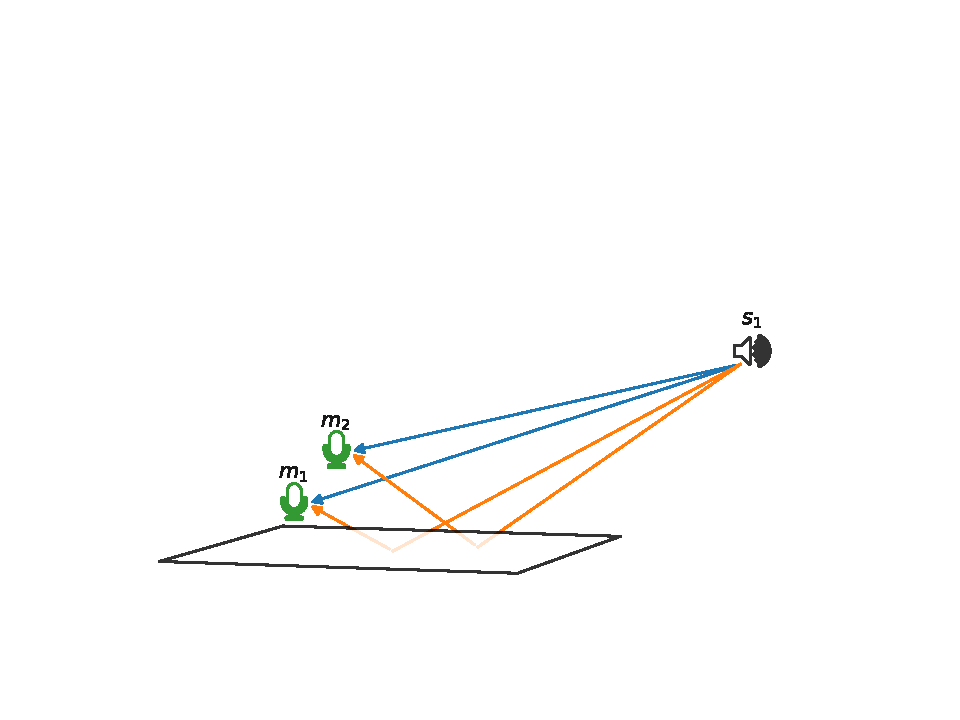
\includegraphics[trim={50 70 50 150},clip,width=\linewidth]{mirage/scene.pdf}
    \captionof{figure}{%
        Typical setup with one source source recorded by two microphones.
        The illustration shows direct sound path (blue lines) and resulting first-order echoes (orange lines).}
    \label{fig:lantern:scene}
}
As a first step, we will use \ac{DNN} to estimate the timings of the first and strongest echo from stereophonic recordings, \ie/ $\numEchs=1$.
To this end, we consider a simple yet common scenario: two microphone placed close to a surface, as illustrated in~\cref{fig:lantern:scene}.
Such a scenario is motivated by the echo-aware \acf{SSL} application that will be discussed in~\cref{ch:mirage}.
The reason why we consider only single microphone pairs is that this approach can be generalized to microphone array using data-fusion-line approaches.
In fact, by considering all the pairs, it is possible to aggregate all their estimation a second moment.\sidenote{
    An example of this approach is the \ac{SRP-PHAT}~\citeonly{dibiase2001robust} algorithm used is \ac{SSL} which uses
    the knowledge of the microphone array geometry to aggregate the contribution of each microphone pair.
}
In the remaining part of this chapter, we will discuss how to achieve robust first-echo estimation and how it could be generalized to multiple echoes.

\subsection{Proposed approach}
Our approach is to train a \ac{DNN} on a dataset simulating the considered close-surface scenario.
Under this assumption and the \acf{STFT} signal model presented in~\cref{eq:processing:stft}, we can consider the following simplified model for the \acfp{RTF},
\begin{equation}\label{eq:mirage:rir}
    \FLT_\idxMic[k] = \sum_{\idxEch=0}^{\numEchs=1}  \; \alpha_\idxMic^{(\idxEch)}[k] \; \cste^{- \csti 2 \pi f_k \tau_\idxMic^{(\idxEch)}} \; + \; \varepsilon_\idxMic[k],
\end{equation}
where $\tau_\idxMic^{(\idxEch)}$ and $\alpha_\idxMic^{(\idxEch)}[k]$ are the echoes's time of arrival and amplitude, respectively.
The $f_k$ denotes $k$-th frequency bin and the error term $\varepsilon_i[k]$ collects later echoes, the reverberation tail, diffusion, and noise.

\mynewline
We model the \AER/ problem as multi-target regression problem, namely the output on the model are multiple real-valued parameters.
Following the approaches suggested in~\citeonly{deleforge2015acoustic,gaultier2017vast}, we consider the instantaneous \acf{ILD} and the \ac{IPD} as input features.
As discussed in~\cref{subsec:processing:steering}, the \ac{ILD} and \ac{IPD} can be consider as a particular case of \acf{ReTF}.
The \ac{ILD} and \ac{IPD} can be estimated from the \STFT/ of the microphone signals, such as,
\begin{equation} \label{eq:mirage:features}
\begin{cases}
    \ild[k]  =& \tfrac{1}{T} \sum_{l=1}^T \log{\abs{\frac{\MIC_2[k,l]}{\MIC_1[k,l]}}}, \\
    \ipd[k]  =& \tfrac{1}{T} \sum_{l=1}^T \frac{\MIC_2k,l]/ \abs{\MIC_2[k,l]}}{ \MIC_2k,l] / \abs{\MIC_1[k,l]}},\\
\end{cases}
\end{equation}
where $\MIC_i[k,l]$ is the \ac{STFT} of the $i$-th microphone.
\\More precisely, the input of the network is
\begin{equation*}
    \xi = \klist{ \ild, \kRe\set{\ipd}, \kIm\set{\ipd}}
    ,
\end{equation*}
namely the concatenation of the above features for all the frequencies.
Here $\kRe\set{\cdot}$ and $\kIm\set{\cdot}$ denote real and imaginary part operators, respectively.
Note that for the \ac{IPD}, the frequency $k=0$ is discarded because it is constant for every observation.

\newcommand{\setTDOA}{\ensuremath{\set{\mathtt{TDOA}, \mathtt{iTDOA}, {\mathtt{TDOE}_1}}}}
\mynewline
Initial investigation shown that learning directly the echoes arrival time and their amplitude yield huge estimation error, probable to the complexity of the task.
Motivated by the application in \ac{SSL} discussed in~\cref{ch:mirage}, we consider only the \acfp{TDOA} between the direct path propagation.
\begin{align}
    \tau_\mathtt{TDOA}  &= \tfrac{1}{c} \norm{\positionMicrophone_2 - \positionSource} - \tfrac{1}{c} \norm{\positionMicrophone_1 - \positionSource} = \tau_2^{(0)} - \tau_1^{(0)} \quad[\text{s}],\\
    \tau_\mathtt{iTDOA} &= \tfrac{1}{c} \norm{\mathring{\positionMicrophone}_2 - \positionSource} - \tfrac{1}{c} \norm{\mathring{\positionMicrophone}_1 - \positionSource} = \tau_2^{(1)} - \tau_1^{(1)} \quad[\text{s}],\\
    \tau_{\mathtt{TDOE},1}  &= \tfrac{1}{c} \norm{\mathring{\positionMicrophone}_1 - \positionSource} - \tfrac{1}{c} \norm{\positionMicrophone_1 - \positionSource} = \tau_1^{(1)} - \tau_1^{(0)} \quad[\text{s}],
\end{align}
where $\mathring{\positionMicrophone}_i$ denotes the position of the image of the microphone at position $\positionMicrophone_i$ with respect to the reflector.
Note that $\tau_{\mathtt{TDOE},2} = \tau_\mathtt{iTDOA} + \tau_{\mathtt{TDOE}, 1} - \tau_\mathtt{TDOA}$.
These three quantities are directly connected to \RIRs/, as illustrated in~\cref{fig:lantern:rirs_tdoa}\marginpar{%
\centering
\footnotesize
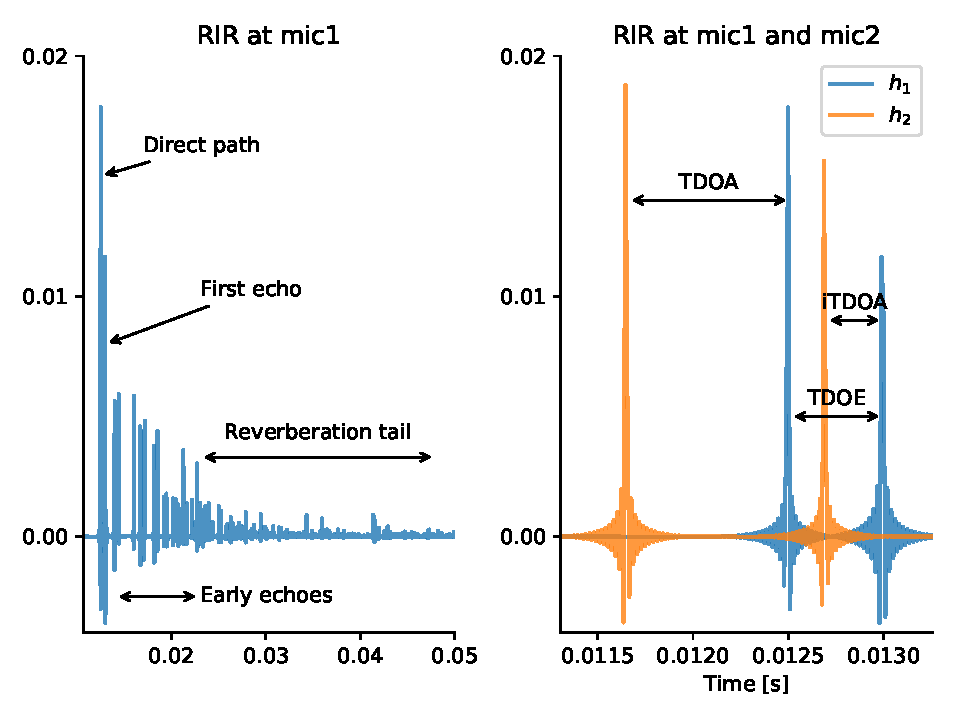
\includegraphics[trim={82mm 0 0 0},clip,width=\linewidth,height=7cm]{mirage/rirs.pdf}
\captionof{figure}{%
    Superposition of two \acp{RIR} and visualization of time difference of arrival between direct paths (\ac{TDOA}), first echoes (\ac{iTDOA}) and direct path and first echo (\ac{TDOE}).}
\label{fig:lantern:rirs_tdoa}
}. Let $V = \klist{\tau_{\mathtt{TDOA}}, \tau_{\mathtt{iTDOA}}, \tau_{\mathtt{TDOE},1}}\in\mathbb{R}^3$ be the vector of the parameters of interest
and $\calV = \setTDOA$ the set of corresponding labels.

\mynewline
Since we use \ReTF/-based feature to estimate echoes, the proposed approach is dubbed as \textit{\acf{LANTERN}}.

\mynewline
In general, the mapping between $V$ and the proposed feature is not unique.
In particular, this happen when $\tau_2^{(\idxEch)} = \tau_1^{(\idxEch)}$ for $\idxEch=\set{0,1}$.
In order to avoid this, we preventively pruned all the entries with $| \tau_2^{(\idxEch)} - \tau_1^{(\idxEch)} | < 10^{-6}$ for $\idxEch=\set{0,1}$ from the dataset.

\mynewline
Here we use the simple \ac{MLP} architecture described in~\cref{subsec:lantern:mlp}.
This model consists of a $D$-dimensional input layer, a 3-dimensional output layer, and 3 fully connected hidden layers with respective input sizes $500$, $300$, and $50$.
\ac{ReLU} activation functions are used except at the output layer, and each hidden layer has a dropout probability $p_\text{do} = 0.3$ to prevent overfitting.
\\We use the \ac{MSE} loss function for training, that is,
\begin{equation}\label{eq:lantern:mlploss}
    \calL_\theta(V, \hat{V)} = \frac{1}{|\calV|} \sum_{\xi\in\Xi} \sum_{v\in\calV} \powerOf{\tau_{v, \xi} - \hat{\tau}_{v, \xi}}
\end{equation}
where $v$ indexes one of \ac{TDOA} in $\calV$, $\xi$ denotes a sample in the mini-batch $\Xi$, and $\theta$ are the model parameters.

\mynewline
The \acf{nRMSE}\sidenote{
    The ac{nRMSE} takes values between $0$ (perfect fit) and $\infty$ (bad fit).
    If it is equal to $1$, then the prediction is no better than a constant.
    It is typically chosen because it is more robust to outliers than \ac{RMSE}.
}is taken as validation metric for assessing the quality of the estimation $\hat{V}$.
The network is manually tuned on a validation set to find the best combination of number of hidden layers, their sizes and $p_\text{do}$.

\subsection{Data, implementation and experimental results}
For training and validation of the \ac{MLP} we generate many random, shoe-box room configurations using the software presented in \citeonly{schimmel2009fast}.
This software implements both the \acf{ISM} for simulating reflections and a ray-tracing algorithm for diffusion.
Room widths are uniformly drawn at random in $[3, 9]$ m, heights in $[2, 4]$ m.
Random source and microphones positions are used, respecting the close-surface scenario.\sidenote{
    A rejection-sampling strategies was used to approximate uniform distributions.
}
In particular, the microphones are at most 30~cm from the close-surface, placed 10~cm from each other, and the other walls' absorption coefficients are uniformly sampled in $(0.5, 1)$ and the one of the close-surface is in $(0, 0.5)$.
The same realistic diffusion profile \citeonly{gaultier2017vast} is used for all surfaces.
Around $90,000$ audio scenes are generated this way, yielding a \ac{RT$_{60}$} between $20$ ms and $250$ ms.
\\The \acp{RIR} are convolved with 1 sec of white-noise (wn) with no additional noise.
All signals and \acp{RIR} are sampled at $16$ kHz.
The \ac{STFT} is performed on $1024$ point with $50\%$ overlap.
Finally the features are computed as in~\eqref{eq:mirage:features} yielding a vector of size $D = 1534$ for each observation.
\\While we validate the \ac{MLP} on a portion of the dataset in a \textit{holdout} fashion, the test is conducted on 200 new \acp{RIR} convolved with both wn and speech (sp) utterances.
This set is generated similarly to the training and validation sets.
Moreover, the test recordings are perturbed by external white noise at 10~dB \acf{SNR} (wn+n, sp+n).
The speech signals are normalized speech utterances of various lengths (from $1$ s to $6$ s), randomly selected from the TIMIT corpus.
% A free and open-source Matlab implementation of SRP-PHAT\footnote{\url{http://bass-db.gforge.inria.fr/bss_locate/}} is used to aggregate local angular spectra obtained from the DNN's output.
% The same toolbox is used for the implementation of SPR-PHAT with GCC-PHAT. For the latter method only real pairs are used.
% A sphere sampling with $\ang{0.5}$ resolution and coordinates $\theta \in [-179, 180]$ and $\phi \in [0, 90]$ is used for the DOA search.

\newthoughtpar{Experimental results}\label{subsec:lantern:mlpdata}
To check the validity of \ac{TDOA} estimation with the proposed \ac{MLP} model, we compare it to a baseline algorithm \acf{GCC-PHAT} (see~\cref{subsec:mirage:1D-SSL}).
\ac{GCC-PHAT} is a popular method for estimating \ac{TDOA} between two microphone recordings.
It is known to achieve good performance in the case of the broadband source signal.
However, it was shown that as soon as the acoustic condition becomes challenging due to strong early echoes, high reverberation level, and noise, the method performances decrease~\citeonly{chen2006time}.

\begin{table}[h]
    \begin{sidecaption}[Echo estimation with MIRAGE results]{%
        Normalize root mean squared error for TDOA estimation using the \ac{MLP} architecture.
    }[tab:lantern:tdoas-aoa]
    \centering
    \footnotesize
    \small
    \begin{tabular*}{\linewidth}{@{\extracolsep{\fill}}lcl|cccc@{}}
    \toprule
    &            &         &          & nRMSE           &\\
    &            & Input   &    \ac{TDOA}  	&   \ac{iTDOA} 		 &     \ac{TDOE}   	&\\
    \midrule
    & MIRAGE      &   wn    & 0.18    & 0.28  & 0.25 	& \\
    & MIRAGE      &   wn+n  & 0.68    & 0.69  & 0.89 	& \\
    & MIRAGE      &   sp    & 0.31    & 0.34  & 0.56    & \\
    & MIRAGE      &   sp+n  & 0.99    & 0.98  & 1.48 	& \\
    & GCC-PHAT    &   wn    & 0.21    & -     & -		& \\
    & GCC-PHAT    &   wn+n  & 0.68    & -     & -		& \\
    & GCC-PHAT    &   sp 	& 0.32    & -     & -		& \\
    & GCC-PHAT    &   sp+n  & 1.38    & -     & -		& \\
    \bottomrule
    \end{tabular*}
    \end{sidecaption}
\end{table}

\mynewline
\ac{TDOA} estimation errors using the proposed approach and \ac{GCC-PHAT} are presented in~\cref{tab:lantern:tdoas-aoa}.
Training a \ac{MLP} to estimate \acp{TDOA} brings similar performances as \ac{GCC-PHAT} in terms of nRMSE.
However, the estimation of \ac{iTDOA} and \ac{TDOE} seems to be a more challenging task for such a simple \ac{MLP} model.
When some external noise is added, the performances of both methods degrades.
This is a well-known and expected behavior for \ac{GCC-PHAT}, and it suggests that noise should also be considered in the training phase. When
Nevertheless, our results confirm the possibility of retrieving the strongest echoes from only two-microphone recordings.

\section{Robustly learning the first echo}\label{sec:lantern:robust}
The above model was proposed in the our published work~\citeonly{di2019mirage}.
To overcome the limitations of such a simple approach with introduced the following three modifications:
\begin{itemize}
    \item use state-of-the-art deep learning architecture;
    \item include corrupting noise in the training data;
    \item and use a robust loss function which is able to return a level of confidence of the estimation.
\end{itemize}
Motivated by their success, we consider a \ac{CNN} architecture (see~\cref{subsec:lantern:cnn}).
To this end, we inspire by the works~\citeonly{chakrabarty2017broadband,nguyen2018autonomous} for the task of \ac{SSL}.
\begin{figure}[h]
    \begin{sidecaption}[CNN]{
        Architecture of the proposed deep neural network. Input and output dimensions for each stage are reported. The first dimension is the batch size $B = 200$.
        }[fig:lantern:cnn]
        \centering
        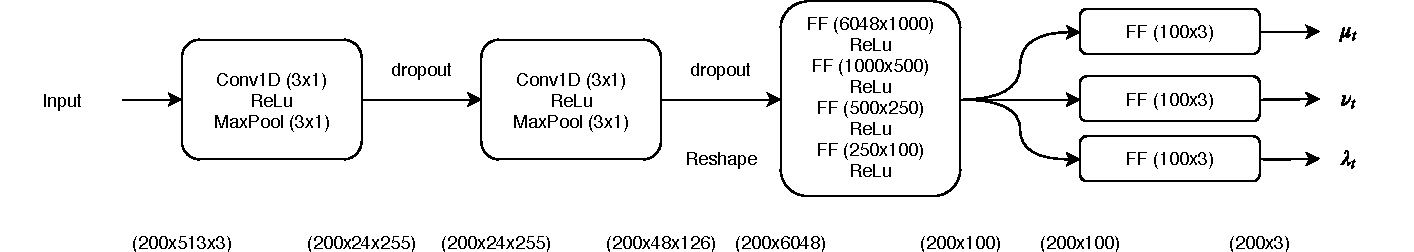
\includegraphics[width=\linewidth]{mirage/cnn.pdf}
    \end{sidecaption}
\end{figure}
As shown in~\cref{fig:lantern:cnn}, the architecture consists of two convolutional modules made of a one-dimensional convolutional layer (1DConv) followed by max-pooling along the frequencies, followed by \ac{ReLU} activation function and batch-normalization.
The second part consists of a cascade of fully connected feed-forward (FF) layers (basically the \ac{MLP} model discussed above).
In order to perform 1D-convolution ond the right dimension, we re-arranged the input so that the each of features $\klist{ \ild, \kRe\set{\ipd}, \kIm\set{\ipd}}$ is considered as channel for the 1DConv.
After each layer a dropout probability $p_\text{do} = 0.3$ is applied to prevent overfitting.

\mynewline
\subsection{Gaussian- and Student's T-based CNNs}
In the \ac{MLP} model presented in the previous section, the output consisted only in the \acp{TDOA} $V$.
As mention earlier, our final goal is to generalize this approach to microphone array in a data-fusion-like fashion.
To this end, we need to provide a confidence measure on the estimate.
In our work~\citeonly{di2019mirage}, we proposed to use predicted values and the error on the validation set as mean and variance to build a Gaussian prior.
Instead, here, we explicitly modify the \ac{CNN} model to estimated these parameters.
This idea recalls Bishop's\ac{MDN} in \citeonly{bishop1994mixture}, where the output of a neural network parametrizes a Gaussian mixture model.
The rationale behind this design choice is to allow the learning model to assess its prediction quality.
In order to achieve this, both loss functions and network outputs need to be modified accordingly.
\newcommand{\xiTheta}{{\xi;\theta}}
\newcommand{\sigmaTauv}{\ensuremath{\sigma^2_{v}(\xiTheta)}}
\newcommand{\muTauv}{\ensuremath{\mu_{v}(\xiTheta)}}
\newcommand{\sigmaTau}{\ensuremath{\sigma^2_{v}}}
\newcommand{\muTau}{\ensuremath{\mu_{v}}}
\newcommand{\estSigmaTau}{\ensuremath{\sigma^2_{v}}}
\newcommand{\estMuTau}{\ensuremath{\mu_{v}}}

\newthought{The Gaussian-based loss function} is derived as follows.\marginpar{
    \footnotesize
    The general form of the Gaussian probability density function is
    \begin{equation*}
        \calN\kparen{x; \mu, \sigma^2} = \frac{1}{\sqrt {2\pi \sigma^2}}
                                         \cste^{-{\frac {1}{2}}\left({\frac {x-\hat{\mu}}{\sigma }}\right)^{2}}
        .
    \end{equation*}
} First, we modify the network to return mean and variances, namely
$V_{\calN} = \set{\muTauv, \sigmaTauv}_v$ for $v = \setTDOA$.
Moreover, we assume that the probability of observing each of the $\tau_v$ for each $v \in \setTDOA$, given the observation $\xi$ in the mini-batch $\Xi$, follows a Gaussian distribution, namely
\begin{equation}
    p(\tau_v \mid  \xi ; \theta) \sim \calN\kparen{\tau_v; \muTauv, \sigmaTauv}
    .
\end{equation}
From now on, we omit the dependency on $(\xiTheta)$ for the sake of clarity.
\\Finally, the corresponding training loss function is the negative Gaussian log-likelihood, that is,
\begin{equation}\label{eq:lantern:gausslog}
    \calL_{\params}^{\calN}(V, \hat{V)} = \frac{1}{\kvbar{\calV}}
                                        \sum_{\xi\in\Xi} \sum_{v\in\calV}
                                                \log{\estSigmaTau}
                                                + \frac{\powerOf{\tau_v - \estMuTau}}{\estSigmaTau}
    .
\end{equation}
It follows that for each each input $\xi$, the network will return the parameters of 3 Gaussian distributions, ($\estMuTau, \estSigmaTau$) for each variable $v\in\calV$.
Moreover, it is easy to see that the estimated \acp{TDOA} values identify with the $\set{\estMuTau}_v$ for each $v\in\calV$.
Hereafter we denote with $\hat{V}_{\calN}$ the set of the six network outputs.
\\This approach can then be generalized to other this of distribution.
For instance, we can consider a Student's \textit{t-distribution}, which is supposed to be more robust to outliers.
Using such distribution has already been proposed in the context of binaural \ac{SSL}, such as~\citeonly{zohny2014modelling,deleforge2016rectified}.

\newthought{The Student's \textit{t}-based loss function}
\marginpar{
    \footnotesize
    The general form of the Student's \textit{t} probability density function is
    \begin{equation*}
        \calT(x; \mu, \lambda, \nu) = \frac{\Gamma(\frac{\nu+1}{2})} {\sqrt{\nu\pi}\,\Gamma(\frac{\nu}{2})} \left(1+\frac{t^2}{\nu} \right)^{\!-\frac{\nu+1}{2}}
        ,
    \end{equation*}
    where $\Gamma(n)=(n-1)!$ is the Gamma function, defined for positive integers.
} can be derived similarly in the Gaussian case assuming a \textit{t}-distribution prior on the prediction.
We will reminds to the~\cref{ap:studentT} for the detailed derivation.
% \newcommand{\nuTauv}{\ensuremath{\nu^2_{\tau_v}(\xiTheta)}}
% \newcommand{\lambdaTauv}{\ensuremath{\lambda^2_{\tau_v}(\xiTheta)}}
% \begin{equation}
%     p(\tau_v \mid  \xi ; \theta) \sim \calT\kparen{\tau_v; \muTauv, \lambdaTauv, \nuTauv}
%     .
% \end{equation}
% \begin{equation}
With that being said, the corresponding loss function is the negative \textit{t}-distribution log-likelihood writes
\begin{equation}
    \begin{split}
    \ \calL_{\params}^{\calT}(V, \hat{V)} =
                         \sum_{\xi\in\Xi} \sum_{v\in \calV}
                        &    \dfrac{1}{2} \log (\nu_v\pi_v)
                           + \dfrac{1}{2} \log(\lambda_v^2)
                           - \log  \Gamma \left( \dfrac{\nu_v+1}{2} \right)\\
                        &  + \log  \Gamma \left( \dfrac{\nu_v}{2} \right)
                           + \dfrac{\nu_v+1}{2} \log \left( 1  + \dfrac{\powerOf{\mu_v - \tau_v)}}{\nu_v \lambda_v^2} \right)\\
    \end{split}
\end{equation}
where $\Gamma$ is the Gamma function.
Similarly to the Gaussian case, at each each input $\xi$, the network will return the parameters of 3 \textit{t}-distribution ($\mu_v, \nu_v, \lambda_v$) for each variable $v\in\calV$.
The set of there nine network output is denoted as $\hat{V}_{\calT}$.

\subsection{Experimental results}
In order to validate the proposed approach, it is compared to the vanilla \ac{MLP} model proposed above in the previous section.
Rather than training on noise-less observation, we consider microphone recordings featuring background noise.
To this end, we perturbed the observed microphone signals with \ac{AWGN}, leading to \ac{SNR} values uniformly distributed in $[0, 30]$~dB.
While, the test set include observation featuring \ac{SNR} level of $[0, 10, 20]$~dB.
The protocol to generate the observations and the feature extraction steps are the same (\cref{subsec:lantern:mlpdata}), but the investigation is restricted to broadband source signal (white noise) only.
The network is manually tuned on a validation set to find the best combination of the number of hidden layers and their sizes.

\mynewline
\cref{fig:lantern:snr10} shows the performances of the proposed models $\mathtt{CNN}_{\calV}$, $\mathtt{CNN}_{\calV_\calN}$ and $\mathtt{CNN}_{\calV_\calT}$ with respect the
$\mathtt{MLP}_{\calV}$ and the baseline $\mathtt{GCC-PHAT}$ of the described in the section for the task of estimating \ac{TDOA}, \ac{iTDOA} and \ac{TDOE}.
Again we report the performance in terms of \ac{nRMSE} computed on the test samples.
\begin{figure}[h]
    \begin{sidecaption}[]{%
        Normalize root mean squared error (the lower, the better) for \ac{TDOA} estimation using the proposed architectures.
    }[fig:lantern:snr10]
    \centering
    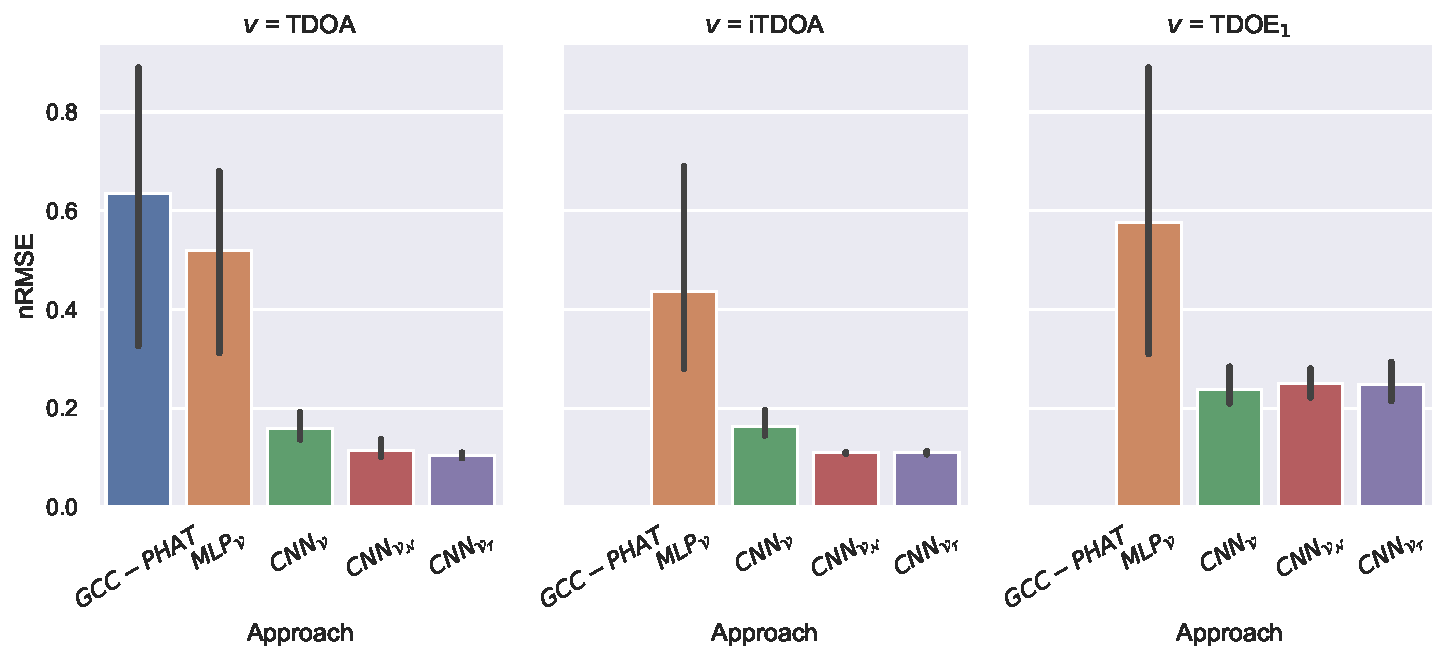
\includegraphics[width=\linewidth]{lantern/snr10.pdf}
    \end{sidecaption}
\end{figure}
It can be seen that the proposed modifications (\ac{CNN}, robust loss function, and considering noise in training) yield considerable improvement in the performance, with respect to the vanilla and baseline methods.
In particular, they are more robust to noise, as indicate by the error bar.
Nevertheless, while both $\mathtt{CNN}_{\calV_\calN}$ and $\mathtt{CNN}_{\calV_\calT}$ outperform the $\mathtt{CNN}_{\calV}$ for \ac{TDOA} and \ac{iTDOA} estimation, it seems there is are no significant differences between them.
\\Deeper insight about this can be envisioned in~\cref{fig:lantern:snr}, where the performances are reported for different \ac{SNR} levels considered at the test phase.
\begin{figure}[h]
    \begin{sidecaption}[]{%
        Normalize root mean squared error (the lower, the better) for \ac{TDOA} estimation using the proposed architectures for different \ac{SNR} levels.
    }[fig:lantern:snr]
    \centering
    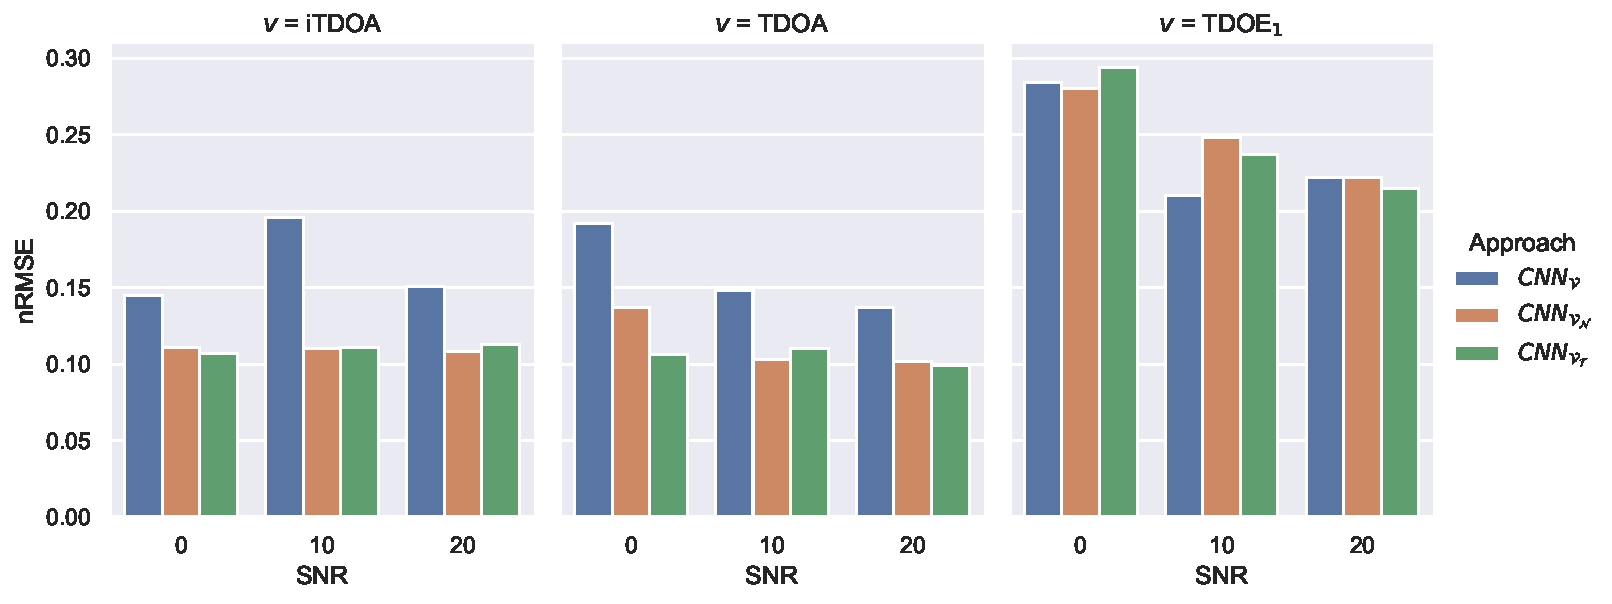
\includegraphics[width=\linewidth]{lantern/snr.pdf}
    \end{sidecaption}
\end{figure}
These results suggest that using a simple \ac{MSE}-based loss function yield to performance more sensitive to external noise.
Besides, again it seems that considering the \textit{i}-distribution do not bring significant difference over the Gaussian-case.
Nevertheless, the choice of modeling the output of the network according to different distributions may lead to differences at the data-fusion step.

\section{Conclusion}\label{sec:lantern:conclusion}
This chapter presented an attempt to use deep learning models to learn the complex mapping from stereophonic recordings to echoes' timings.
As part of a fist investigation, we consider a simple yet common scenario where two microphones are placed close to a surface and listen to a single source's sound.
Moreover, the proposed approach is limited to estimating the time delays between the two microphones, the direct propagation path, and the first-strongest reflection.
This simplification is motivated by an application to echo-aware \ac{SSL}, which will be presented in~\cref{ch:mirage}.
\\We studied two standard \ac{DNN} architectures, which are trained in virtually supervised fashion with data generated by an acoustic simulator.
Finally, we discuss three ways to increase such performances, \ie/, training on noisy data, using the \ac{CNN} architecture, and use robust loss functions.
\\The investigation so far was limited to microphone pairs.
Taking inspiration from data-fusion approaches, in chapter~\cref{ch:mirage}, we will propose to aggregate to multiple pairs' contributions together to improve the final estimation.
To this end, we modify the output of the \ac{DNN} in order to return a confidence measure.

\mynewline
A nature follow-up of this work could consider the following directions.
\begin{itemize}
    \item The first direction consider the generalization to to more reflections.
    Unfortunately this step is not trivial.
    Current informal investigation spanned different training paradigm, such as, \textit{curriculum learning}~\citeonly{bengio2009curriculum}, \textit{teacher-student learning}~\citeonly{tu2019speech}, where the network is subsequently trained to estimate more echoes.
    Other approaches are currently subject of investigation, such as, using a combination of \acs{DNN} pre-trained for single echo estimation.
    \item Due to the drop of performances when using speech signals, we could consider more robust audio features (\eg/, \ReTF/ using state-of-the-art \ReTF/ estimators) or
    \ac{DNN} architecture designed to handle missing input data.
    \item Finally, another interesting direction comes from physics-driven neural networks~\citeonly{nabian2020physics,rao2020physics,jin2020physics},
    where physical-based layers or physically-motivated regularizers are implemented facilities the learning.
\end{itemize}

% \begin{table}[ht!]
%     \begin{sidecaption}[Echo estimation with MIRAGE results]{%
%         Normalize root mean squared error for TDOA estimation and mean angular error in ${}^\circ$ (with accuracies ($\%$))
%         for AOA estimation with $\ang{10}$ and $\ang{20}$ angular tolerance.
%     }[tab:mirage:tdoas-aoa]
%     \centering
%     \footnotesize
%     %\scriptsize
%     \begin{tabular}{cl|ccc|cc}
%     \toprule
%                 &         &          & nRMSE        &                   &\multicolumn{2}{c}{ACCURACY}  \\
%                 & Input   &    \scriptsize{TDOA}  	&   \scriptsize{iTDOA} 		 &     \scriptsize{TDOE} 		 & $\theta<\ang{10}$ &  $\theta<\ang{20}$ \\
%     \midrule
%     MIRAGE      &   wn    & 0.18    & 0.28  & 0.25 	& 4.10 (77)	& 5.97 (97) \\
%     MIRAGE      &   wn+n  & 0.68    & 0.69  & 0.89 	& 5.00 (26)	& 9.89 (54) \\
%     MIRAGE      &   sp    & 0.31    & 0.34  & 0.56  & 4.83 (63)	& 7.26 (82) \\
%     MIRAGE      &   sp+n  & 0.99    & 0.98  & 1.48 	& 4.60 (16)	& 9.88 (35) \\
%     GCC-PHAT    &   wn    & 0.21    & -     & -		& 4.22 (81) & 6.19 (97) \\
%     GCC-PHAT    &   wn+n  & 0.68    & -     & -		& 4.03 (65) & 5.34 (83) \\
%     GCC-PHAT    &   sp 	  & 0.32    & -     & -		& 4.08 (82) & 5.34 (97) \\
%     GCC-PHAT    &   sp+n  & 1.38    & -     & -		& 4.70 (19) & 8.38 (32) \\
%     \bottomrule
%     \end{tabular}
%     \end{sidecaption}
% \end{table}